\documentclass[letterpaper,10pt,onecolumn]{article}
\usepackage[spanish]{babel}
\usepackage[utf8x]{inputenc}
\usepackage{amsfonts}
\usepackage{amsthm}
\usepackage{amsmath}
\usepackage{mathrsfs}
\usepackage{empheq}
\usepackage{enumitem}
\usepackage[pdftex]{color,graphicx}
\usepackage{hyperref}
\usepackage{listings}
\usepackage{calligra}
\usepackage{algpseudocode} 
\DeclareMathAlphabet{\mathcalligra}{T1}{calligra}{m}{n}
\DeclareFontShape{T1}{calligra}{m}{n}{<->s*[2.2]callig15}{}
\newcommand{\scripty}[1]{\ensuremath{\mathcalligra{#1}}}
\lstloadlanguages{[5.2]Mathematica}
\setlength{\oddsidemargin}{0cm}
\setlength{\textwidth}{490pt}
\setlength{\topmargin}{-40pt}
\addtolength{\hoffset}{-0.3cm}
\addtolength{\textheight}{4cm}

\begin{document}
\begin{center}



\includegraphics[width=490pt]{header.png}\\[0.5cm]

\textsc{\LARGE Taller 7 - F\'isica I (FISI-1018) - 2016-10}\\[0.5cm]

\textsc{\Large{Profesor: Jaime Forero}} \\[0.5cm]

\noindent\textsc{Ejercicios correspondiente a la clase complementaria de la semana del 7 de Marzo del 2016.}\\[0.5cm]
\end{center}

\noindent\textsc{Nota:} 
Los primeros tres ejercicios deben ser
entregados {\bf al comienzo} de la clase complementaria. Los \'ultimos
cuatro deben ser trabajados {\bf durante} la complementaria. 

La numeraci\'on
hace referencia al texto gu\'ia: \textit{F\'isica Universitaria Volumen
  1 (Sears-Semansky)}, decimotercera edici\'on, Pearson.

\begin{enumerate}

% aqui vienen los tres ejercicios "faciles"
\item Ejercicio 6.7 Dos bloques conectados por una cuerda. %Juan Carlos
\item Un bloque de $25kg$ de masa es  arrastrado $3.5m$ a lo largo de una superficie horizontal sin fricción, por una  fuerza constante de $100N$  dirigida a $40^{\circ}$ con la horizontal. Encuentre el  trabajo efectuado por la componente paralela y perpendicular de la fuerza.
%Miguel
\item Ejercicio 6.44 La mitad de un resorte.

% aqui vienen los cuatro ejercicios "dificiles"
\item Ejercicio 6.71 Un objeto atraído hacie el origen. %Juan Carlos

\item una partícula de $10kg$  se desplaza en el eje $z$ y su posición esta dada por la ecuación $z=\frac{3}{2}t+4t^3$. Determine en función de $t$.
\begin{enumerate}
\item energía cinética. 
\item La fuerza que actúa sobre ella y su aceleración. 
\item La potencia de la fuerza. 
\item El trabajo entre $t=0s$ y $t=2s$.
\end{enumerate}
 %Miguel
\item Problema 6.75 Bloque con cuerda sobre una mesa.
\item Problema 6.78 Hombre y bicicleta.
 \end{enumerate}
 

\end{document}


\begin{figure}[h]
\begin{center} 
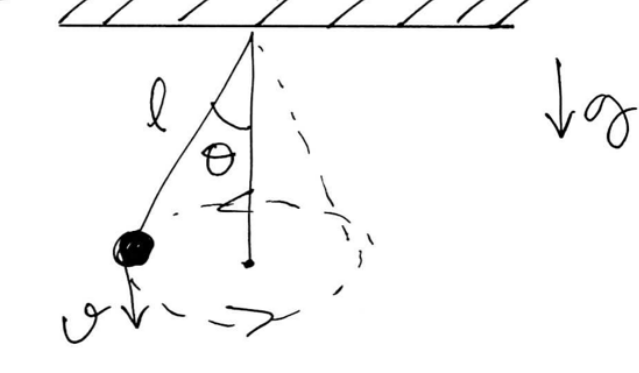
\includegraphics[scale=0.25]{conico.png} 
\caption{\label{fig:conico}Figure para el problema \ref{conico}}
\end{center} 
\end{figure}

\begin{figure}[!h]
\begin{center}
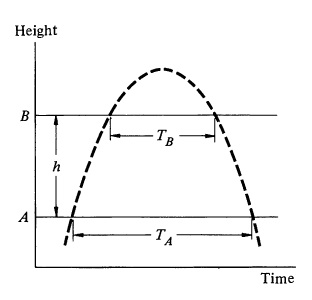
\includegraphics[scale=0.7]{altura.jpg} 
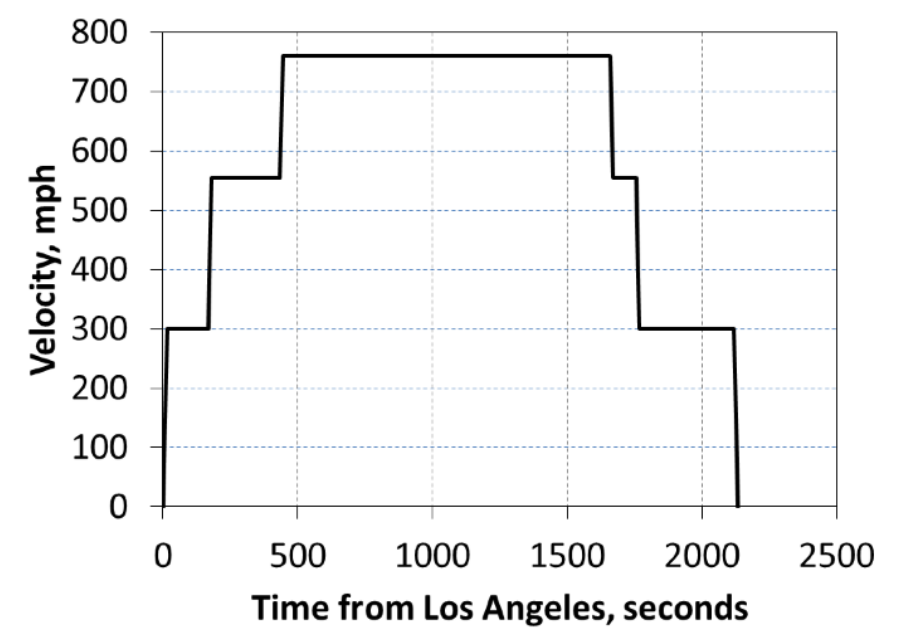
\includegraphics[scale=0.3]{hyperloop.png} 
\end{center}
\caption{Izquierda: diagrama para el ejercicio recomendado 3. Derecha: diagrama para el ejercicio recomendado 4.}
\label{fig:tiro}
\end{figure}





